\documentclass[12pt]{article}
\usepackage[left=3cm, top=1cm, right=3cm, bottom=3cm]{geometry}
\usepackage[utf8]{inputenc}      % accents dans le source
\usepackage[T1]{fontenc}
\usepackage[french]{babel}
\usepackage{graphicx}
\usepackage{graphics}
\usepackage{amsmath}
\usepackage{tikz}
\usepackage{xcolor} 
\usepackage{mathtools}
\usepackage{parskip}
\usepackage{subcaption}
\usepackage[export]{adjustbox}
\usepackage{chemist}
\usepackage{rotating}
\usepackage{hyperref}
\hypersetup{colorlinks=true,linkcolor=blue}

\title{\textbf{TP Cinétique} \\Étude cinétique de la réaction entre le bleu de bromophénol et l'ion hydroxyde}
\author{MENARD Alexandre \\ VIEILLEDENT Florent}

\begin{document}
\maketitle

\section*{Introduction}
Dans ce travail pratique on étudie la cinétique de la réaction entre le bleu de bromophénol et l'hydroxyde.
On suit l'avancement de la réaction par spectrophotomètrie.

\section{Température ambiante}

\textbf{Question 1 :} On calcule la concentration initiale de la solution en BBP. 
La solution utilisée est à $0.4 \ g.L^{-1}$ ce qui correspond à $C_0=5.97\times 10^{-4} \ mol.L^{-1}$, la masse molaire du BBP étant de $669.5 \ g.mol^{-1}$.
On dilue 2 mL de cette solution dans une solution d'hydroxyde qu'on étent à 50mL, on a donc $C=\frac{C_0 \times V_0}{V}=\frac{5.97\times 10^{-4}\times 2}{50}=2.39\times 10^{-5}\ mol.L^{-1}$.

\textbf{Question 2 :} On a pour l'incertitude :
\begin{align*}
    \Delta C &= C \times \left( \frac{\Delta C_0}{C_0} + \frac{\Delta V_0}{V_0} + \frac{\Delta V}{V} \right) \\
    \Delta C &= 2.93\times 10^{-5} \times \left( 0.005 + 0.004 + 0.001 \right) \\
    \Delta C &= 3\times 10^{-7} \ mol.L^{-1}
\end{align*}

\textbf{Question 3 :} On a finalement $C= 2.93 \pm 0.03 \times 10^{-5}\ mol.L^{-1}$.

\textbf{Question 4 :} La solution utilisée pour régler le zéro d'absorbance est la solution d'hydroxyde à $1.4 \ mol.L^{--1}$.

\textbf{Question 5 :} On mesure la température de la pièce à $T_1 = 24 \pm 2 ^\circ C$. 
L'incertitude sur la température est donnée par la thermomètre et le fait qu'on ne contrôle pas la température de la pièce pendant l'expérience.

\textbf{Question 6 :} On mesure pour notre premier une absorbance $A_0=1.15\pm 0.02$. L'incertitude est donnée par le spectrophotomètre et en prenant en compte que l'absorbance varie rapidement au début de l'expérience.
Cette valeur est obtenue pour un temps de 45 secondes, la concentration de BBP a eu le temps de diminuer significativement notre valeur de $\epsilon_{\lambda Bmax}$ ne sera donc pas très précise.
Pour obtenir une valeur plus précise il faut extrapoler nos données jusqu'à $t=0$.
D'après la loi de Beer-Lambert, en utilisant une cuve de 1 cm :
\begin{align*}
    \epsilon_{\lambda Bmax} &= \frac{A_0}{C} \\
    \epsilon_{\lambda Bmax} &= \frac{1.15}{2.93\times 10^{-5}} \\
    \epsilon_{\lambda Bmax} &= 3.93 \times 10^4 \ L.mol^{-1}.cm^{-1}
\end{align*}

\textbf{Question 7 :} On calcule l'incertitude :
\begin{align*}
    \Delta  \epsilon_{\lambda Bmax} &=  \epsilon_{\lambda Bmax} \times \left(\frac{\Delta C}{C} + \frac{\Delta A}{A} \right) \\
    \Delta  \epsilon_{\lambda Bmax} &=  3.93 \times 10^4 \times \left( \frac{0.03}{2.93} \frac{0.02}{1.15}  \right) \\
    \Delta  \epsilon_{\lambda Bmax} &= 0.1 \times 10^4 \ L.mol^{-1}.cm^{-1}
\end{align*}

\textbf{Question 8 :} On a $\epsilon_{\lambda Bmax} =4.0 \pm 0.1 \times 10^4 \ L.mol^{-1}.cm^{-1}$.

\textbf{Question 9 :} Pour trouver la concentration en tout instant on utlise la relation : $[BBP](t)=\frac{A(t)}{\epsilon_{\lambda Bmax}}=\frac{A(t)\times C}{A_0}$.
On prend une incertitude sur le temps de 2 secondes.
\begin{table}[h!]
\begin{center}
    \begin{tabular}{|c|c|c|}
        \hline
        \$Absorbance \textbackslash pm 0.02 \$ & Concentration en mol/L & Temps \textbackslash pm 0.033 en min \\
        \hline
                          1.15 &                   0.00 &                   0.01 \\
                          1.09 &                   0.00 &                   1.07 \\
                          1.05 &                   0.00 &                   2.27 \\
                          1.02 &                   0.00 &                   2.75 \\
                          0.96 &                   0.00 &                   3.47 \\
                          0.92 &                   0.00 &                   4.08 \\
                          0.86 &                   0.00 &                   4.83 \\
                          0.81 &                   0.00 &                   5.47 \\
                          0.77 &                   0.00 &                   6.28 \\
                          0.75 &                   0.00 &                   7.17 \\
                          0.67 &                   0.00 &                   9.00 \\
                          0.62 &                   0.00 &                  10.02 \\
                          0.58 &                   0.00 &                  10.92 \\
                          0.55 &                   0.00 &                  11.97 \\
                          0.51 &                   0.00 &                  12.88 \\
                          0.44 &                   0.00 &                  13.78 \\
                          0.39 &                   0.00 &                  15.33 \\
                          0.36 &                   0.00 &                  16.70 \\
                          0.33 &                   0.00 &                  17.93 \\
                          0.31 &                   0.00 &                  20.98 \\
                          0.29 &                   0.00 &                  21.92 \\
                          0.27 &                   0.00 &                  23.17 \\
                          0.25 &                   0.00 &                  25.27 \\
        \hline
        \end{tabular}
        \caption{Tableau des valeurs de la concentration et de l'absorbance pour les différents temps}
        \label{table1}
\end{center}
\end{table}
\textbf{Question 10:}
On trace [BBP], $ln \left(\frac{[BBP]}{[BBP]_0}\right)$ et $\frac{1}{[BBP]}$ en fonction du temps.

\begin{figure}[h!]
    \begin{center}
        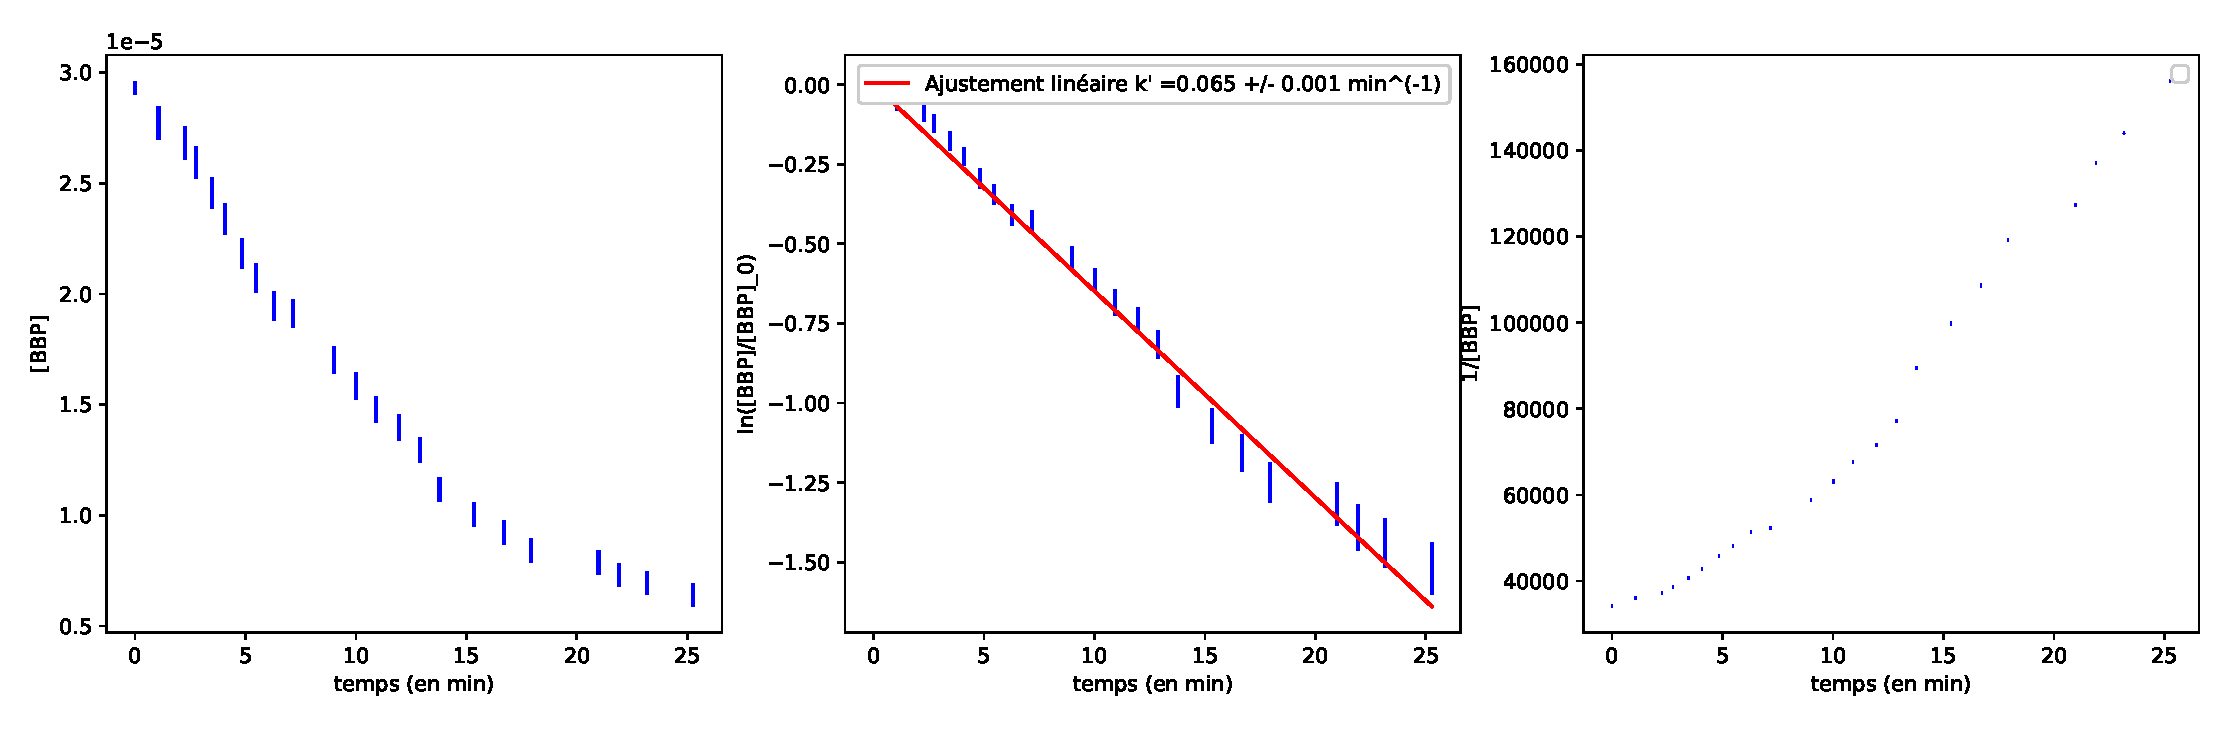
\includegraphics[width=1\linewidth]{3CourbesCinétiques.eps}
        \caption{Courbes de gauche à droite : [BBP], $ln \left(\frac{[BBP]}{[BBP]_0}\right)$ et $\frac{1}{[BBP]}$ en fonction du temps. On a rajouté l'ajustement linéaire pour la deuxième courbe}
        \label{img:3courbes}
    \end{center}
\end{figure}

On remarque qu'on obtient une droite lorsqu'on trace le logarithme.
On a donc l'ordre partiel $\alpha =1$ et on trouve $k'=0.064 \pm 0.001 min^{61}$.

\textbf{Question 11 :}

\end{document}